% vim: set textwidth=120:

% Example CV based on the 1.5-column-cv template. Main features:
% * uses the Roboto font family and IcoMoon icon set;
% * doesn't use colours, different font weights are used instead for styling;
% * because the CV fits on one page, header and footer is empty, since there isn't much useful info to put there;
% * includes a photo.
\documentclass[a4paper,10pt]{article}


% package imports
% ---------------

\usepackage[spanish]{babel} % for correct language and hyphenation and stuff
\usepackage{calc}           % for easier length calculations (infix notation)
\usepackage{enumitem}       % for configuring list environments
\usepackage{fancyhdr}       % for setting header and footer
\usepackage{fontspec}       % for fonts
\usepackage{geometry}       % for setting margins (\newgeometry)
\usepackage{graphicx}       % for pictures
\usepackage{microtype}      % for microtypography stuff
\usepackage{xcolor}         % for colours
\usepackage{outlines}
\usepackage{roboto}
\usepackage{fontspec}
% margin and column widths
% ------------------------

% margins
\newgeometry{left=15mm,right=15mm,top=15mm,bottom=15mm}

% width of the gap between left and right column
\newlength{\cvcolumngapwidth}
\setlength{\cvcolumngapwidth}{3.5mm}

% left column width
\newlength{\cvleftcolumnwidth}
\setlength{\cvleftcolumnwidth}{44.5mm}

% right column width
\newlength{\cvrightcolumnwidth}
\setlength{\cvrightcolumnwidth}{\textwidth-\cvleftcolumnwidth-\cvcolumngapwidth}

% set paragraph indentation to 0, because it screws up the whole layout otherwise
\setlength{\parindent}{0mm}


% style definitions
% -----------------
% style categories explanation:
% * \cvnameXXX is used for the name;
% * \cvsectionXXX is used for section names (left column, accompanied by a horizontal rule);
% * \cvtitleXXX is used for job/education titles (right column);
% * \cvdurationXXX is used for job/education durations (left column);
% * \cvheadingXXX is used for headings (left column);
% * \cvmainXXX (and \setmainfont) is used for main text;
% * \cvruleXXX is used for the horizontal rules denoting sections.

% font families
\defaultfontfeatures{Ligatures=TeX} % reportedly a good idea, see https://tex.stackexchange.com/a/37251

\newfontfamily{\cvnamefont}{Roboto Medium}
\newfontfamily{\cvsectionfont}{Roboto Medium}
\newfontfamily{\cvtitlefont}{Roboto Regular}
\newfontfamily{\cvdurationfont}{Roboto Light Italic}
\newfontfamily{\cvheadingfont}{Roboto Regular}
\setmainfont{Roboto Light}

% colours
\definecolor{cvnamecolor}{HTML}{000000}
\definecolor{cvsectioncolor}{HTML}{000000}
\definecolor{cvtitlecolor}{HTML}{000000}
\definecolor{cvdurationcolor}{HTML}{000000}
\definecolor{cvheadingcolor}{HTML}{000000}
\definecolor{cvmaincolor}{HTML}{000000}
\definecolor{cvrulecolor}{HTML}{000000}

\color{cvmaincolor}

% styles
\newcommand{\cvnamestyle}[1]{{\Large\cvnamefont\textcolor{cvnamecolor}{#1}}}
\newcommand{\cvsectionstyle}[1]{{\normalsize\cvsectionfont\textcolor{cvsectioncolor}{#1}}}
\newcommand{\cvtitlestyle}[1]{{\large\cvtitlefont\textcolor{cvtitlecolor}{#1}}}
\newcommand{\cvdurationstyle}[1]{{\small\cvdurationfont\textcolor{cvdurationcolor}{#1}}}
\newcommand{\cvheadingstyle}[1]{{\normalsize\cvheadingfont\textcolor{cvheadingcolor}{#1}}}


% inter-item spacing
% ------------------

% vertical space after personal info and standard CV items
\newlength{\cvafteritemskipamount}
\setlength{\cvafteritemskipamount}{5mm plus 1.25mm minus 1.25mm}

% vertical space after sections
\newlength{\cvaftersectionskipamount}
\setlength{\cvaftersectionskipamount}{2mm plus 0.5mm minus 0.5mm}

% extra vertical space to be used when a section starts with an item with a heading (e.g. in the skills section),
% so that the heading does not follow the section name too closely
\newlength{\cvbetweensectionandheadingextraskipamount}
\setlength{\cvbetweensectionandheadingextraskipamount}{1mm plus 0.25mm minus 0.25mm}


% intra-item spacing
% ------------------

% vertical space after name
\newlength{\cvafternameskipamount}
\setlength{\cvafternameskipamount}{3mm plus 0.75mm minus 0.75mm}

% vertical space after personal info lines
\newlength{\cvafterpersonalinfolineskipamount}
\setlength{\cvafterpersonalinfolineskipamount}{2mm plus 0.5mm minus 0.5mm}

% vertical space after titles
\newlength{\cvaftertitleskipamount}
\setlength{\cvaftertitleskipamount}{1mm plus 0.25mm minus 0.25mm}

% value to be used as parskip in right column of CV items and itemsep in lists (same for both, for consistency)
\newlength{\cvparskip}
\setlength{\cvparskip}{0.5mm plus 0.125mm minus 0.125mm}

% set global list configuration (use parskip as itemsep, and no separation otherwise)
\setlist{parsep=0mm,topsep=0mm,partopsep=0mm,itemsep=\cvparskip}


% CV commands
% -----------

% creates a "personal info" CV item with the given left and right column contents, with appropriate vertical space after
% @param #1 left column content (should be the CV photo)
% @param #2 right column content (should be the name and personal info)
\newcommand{\cvpersonalinfo}[2]{
    % left and right column
    \begin{minipage}[t]{\cvleftcolumnwidth}
        \vspace{0mm} % XXX hack to align to top, see https://tex.stackexchange.com/a/11632
        \raggedleft #1
    \end{minipage}% XXX necessary comment to avoid unwanted space
    \hspace{\cvcolumngapwidth}% XXX necessary comment to avoid unwanted space
    \begin{minipage}[t]{\cvrightcolumnwidth}
        \vspace{0mm} % XXX hack to align to top, see https://tex.stackexchange.com/a/11632
        #2
    \end{minipage}

    % space after
    \vspace{\cvafteritemskipamount}
}

% typesets a name, with appropriate vertical space after
% @param #1 name text
\newcommand{\cvname}[1]{
    % name
    \cvnamestyle{#1}

    % space after
    \vspace{\cvafternameskipamount}
}

% typesets a line of personal info beginning with an icon, with appropriate vertical space after
% @param #1 parameters for the \includegraphics command used to include the icon
% @param #2 icon filename
% @param #3 line text
\newcommand{\cvpersonalinfolinewithicon}[3]{
    % icon, vertically aligned with text (see https://tex.stackexchange.com/a/129463)
    \raisebox{.5\fontcharht\font`E-.5\height}{\includegraphics[#1]{#2}}
    % text
    #3

    % space after
    \vspace{\cvafterpersonalinfolineskipamount}
}

% creates a "section" CV item with the given left column content, a horizontal rule in the right column, and with
% appropriate vertical space after
% @param #1 left column content (should be the section name)
\newcommand{\cvsection}[1]{
    % left and right column
    \begin{minipage}[t]{\cvleftcolumnwidth}
        \raggedleft\cvsectionstyle{#1}
    \end{minipage}% XXX necessary comment to avoid unwanted space
    \hspace{\cvcolumngapwidth}% XXX necessary comment to avoid unwanted space
    \begin{minipage}[t]{\cvrightcolumnwidth}
        \textcolor{cvrulecolor}{\rule{\cvrightcolumnwidth}{0.3mm}}
    \end{minipage}

    % space after
    \vspace{\cvaftersectionskipamount}
}

% creates a standard, multi-purpose CV item with the given left and right column contents, parskip set to cvparskip
% in the right column, and with appropriate vertical space after
% @param #1 left column content
% @param #2 right column content
\newcommand{\cvitem}[2]{
    % left and right column
    \begin{minipage}[t]{\cvleftcolumnwidth}
        \raggedleft #1
    \end{minipage}% XXX necessary comment to avoid unwanted space
    \hspace{\cvcolumngapwidth}% XXX necessary comment to avoid unwanted space
    \begin{minipage}[t]{\cvrightcolumnwidth}
        \setlength{\parskip}{\cvparskip} #2
    \end{minipage}

    % space after
    \vspace{\cvafteritemskipamount}
}

% typesets a title, with appropriate vertical space after
% @param #1 title text
\newcommand{\cvtitle}[1]{
    % title
    \cvtitlestyle{#1}

    % space after
    \vspace{\cvaftertitleskipamount}
    % XXX need to subtract cvparskip here, because it is automatically inserted after the title "paragraph"
    \vspace{-\cvparskip}
}


% header and footer
% -----------------

% set empty header and footer
\pagestyle{empty}



% preamble end/document start
% ===========================

\begin{document}


% personal info
% -------------

% \cvpersonalinfo{
    % photo
  % 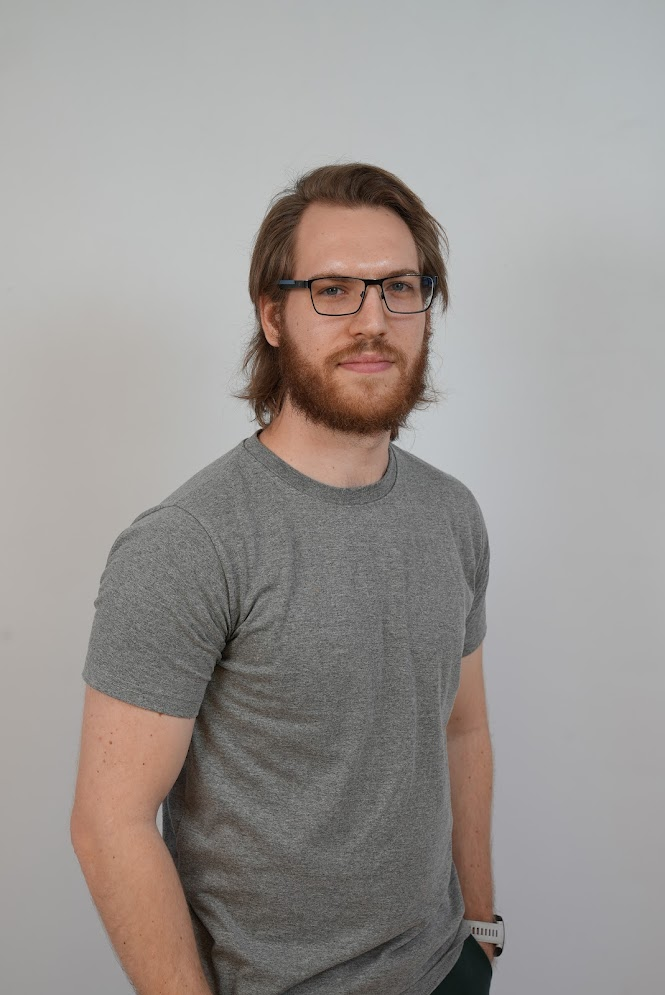
\includegraphics[trim={0 7cm 0 5cm},clip,height=36mm]{../logos-photos/photo-JIT-2023.jpg}
% }{
  \flushright
    % name
    \cvname{Teich, Juan Ignacio}

    % address
    \cvpersonalinfolinewithicon{height=4mm}{../logos-photos/072-location.pdf}{
       Buenos Aires, Argentina
    }

    % phone number
    \cvpersonalinfolinewithicon{height=4mm}{../logos-photos/067-phone.pdf}{
        +54 11\,6491\,6389
    }

    % email address
    \cvpersonalinfolinewithicon{height=4mm}{../logos-photos/070-envelop.pdf}{
        juanignacioteich@gmail.com
    }

    % % LinkedIn account
    % \cvpersonalinfolinewithicon{height=4mm}{458-linkedin.pdf}{
    %     fake-name-123456789
    % }

    % date of birth
        22-03-1999  ---   24 years
% }

% work experience
% ---------------
\cvsection{PROFESSIONAL OBJECTIVES}

\vspace{\cvbetweensectionandheadingextraskipamount}
\cvitem{\cvheadingstyle{}}{
    To continue my professional career, pursuing challenging projects and applying the skills acquired in my academic
    journey.

    I aim to focus on simulation and it's development to adress and better understand industry problems.
}


\cvsection{WORK EXPERIENCE}

\cvitem{
	\begin{minipage}{\textwidth}
    \begin{flushright}
		  % \centering
      % \vfill
		  
\includegraphics[height=0.15\textwidth]{../logos-photos/Logo_STAMM.png}   
	    % \vfill
    \end{flushright}  
  \end{minipage} \\
  \vspace{0.3cm}
  \cvdurationstyle{October 2023 -- Present}\\
}{
	
  \cvtitle{Numerical Simulations Specialist}
  \textbf{\large STÄMM Biotech}
  
  Responsabilities:
  \begin{itemize}
    \item Enhance meshing strategies for complex repetitive structures. 
    \item Develop and run CFD simulations to validate and further improve existing in-house indirect simulation models.
    \item Elaborate post-processing scripts, for various types of OpenFOAM simulations and python simulation scripts.
    \item Formulate OOP code to further develop in-house indirect simulation model.
  \end{itemize}
  
  Skills and tools:
  \begin{itemize}
    \item OpenFOAM, Code\_Saturne, snappyHexMesh, Salome Geometry and Meshing modules, Python, Object Oriented
      Programming, Bash, Linux 
  \end{itemize}
	
}

\cvitem{
 	\begin{minipage}{\textwidth}
   \begin{flushright}
		  % \centering
      % \vfill
		  
\includegraphics[width=0.6\textwidth]{../logos-photos/Logo_SG.png}   
	    % \vfill
    \end{flushright}  
  \end{minipage} \\
  \vspace{0.3cm}
  \cvdurationstyle{November 2022 -- October 2023}
}{
    \cvtitle{Junior Project Engineer}

    \textbf{\large Saint-Gobain Argentina}
	
  Responsabilities	
    \begin{itemize}
        \item Lead strategic projects, including analyzing the company's needs for business continuity, basic project
          design, and implementation.
        \item Coordinate multidisciplinary teams and stakeholders, seeking consensus solutions within scope, time, and
          available budget.
        \item Provide technical support and analysis for acquisitions of new businesses at regional level. 
    \end{itemize}
	
	Skills and tools:
	\begin{itemize}
		\item AutoCAD, SolidWorks, MS Excel, MS PowerPoint, MS Planner, MS Project.
	\end{itemize}

}

% Fake Company 2
\cvitem{
 	\begin{minipage}{\textwidth}
   \begin{flushright}
		  % \centering
      % \vfill
		  
\includegraphics[height=0.25\textwidth]{../logos-photos/Logo_FIUBA_new.png}   
	    % \vfill
    \end{flushright}  
  \end{minipage} \\
  \vspace{0.1cm}
  \cvdurationstyle{March 2020 -- March 2021}
}{
    \cvtitle{Teaching Assistant in Thermodynamics course}

    \textbf{\large Faculty of Engineering, University of Buenos Aires}

    Mechanical Engienering Department
}



% education
% ---------

\cvsection{EDUCATION}

% master's
\cvitem{
 	\begin{minipage}{\textwidth}
   \begin{flushright}
		  % \centering
      % \vfill
		  
\includegraphics[height=0.25\textwidth]{../logos-photos/Logo_FIUBA_new.png}   
	    % \vfill
    \end{flushright}  
  \end{minipage} \\
  \vspace{0.1cm}
  \cvdurationstyle{2017 -- Present}
}{
  \cvtitle{Mechanical Engineering}

    Faculty of Engineering, University of Buenos Aires
    
    \begin{itemize}[leftmargin=*]
       \item \textsf{Thesis in progress - Parametric analysis of disk actuators models to simulate wind farms.} 
        \begin{itemize}
          \item CSC - CONICET - Argentina.
          \item Director: Alejandro Otero, PhD.
          \item Co-Director: Dimas Barile.
        \end{itemize}
        \item Thesis end date: august 2024.    
    \end{itemize}
}


% bachelor's
\cvitem{
    \begin{minipage}{\textwidth}
        \flushright
        
\includegraphics[height=0.2\textwidth]{../logos-photos/Logo_HC.png}   
    \end{minipage}\\  
    \vspace{0.1cm}
    \cvdurationstyle{2011 -- 2016}
}{
    \cvtitle{Bilingual High School}

    Colegio Holy Cross
}

\cvsection{COURSES}

%curso
\cvitem{
    \begin{minipage}{\textwidth}
        \flushright
        
\includegraphics[height=0.15\textwidth]{../logos-photos/Logo_edx.png}   
    \end{minipage}\\
    \vspace{0.1cm}
    \cvdurationstyle{Sep. 2021 -- Nov. 2021}
}{
    \cvtitle{A Hands-on Introduction to Engineering Simulations}
    edX \& Cornell University

    \begin{itemize}
        \item ANSYS course
    \end{itemize}
}
% skills
% ------
% \newpage
\cvsection{SKILLS}

\vspace{\cvbetweensectionandheadingextraskipamount}

% languages
\cvitem{
    \cvheadingstyle{Languages}
}{
    English - fluent 
    \begin{itemize}
        \item IGCSE Certificates, Universidad de Cambridge
    \end{itemize}

    French -  basic
    \begin{itemize}
        \item A1 and A2 certificates
    \end{itemize}
}

%software
\cvitem{
    \cvheadingstyle{Software}
}{
    Autodesk Fusion 360
    
    MS Office (Excel, Word, PowerPoint, Project)

    AutoCAD
    
    ANSYS
    
    LaTeX 
    
    OpenFoam

    MatLab

    SolidWorks

    Linux

    Python

    Object Oriented Programming

    Code\_Saturne

    Salome Geometry and Meshing Modules
}


%\cvsection{INTERESES PERSONALES}

%\vspace{\cvbetweensectionandheadingextraskipamount}
%\cvitem{\cvheadingstyle{}}{
%    Tengo interés por los deportes en general, en partícular realizo rutinas de musculación en un gimnasio y he realizado múltiples deportes de equipo e individuales en el pasado.
%
%    Soy un aficionado de la lectura, en particular de fantasía, ciencia-ficción, crimen y suspenso.
%}

% fake skills
% \cvitem{
%     \cvheadingstyle{Fake skills}
% }{
%     Fake skill 1
%     \begin{itemize}
%         \item fake skill description (excepteur sint occaecat cupidatat non proident)
%         \item fake skill details (sunt in culpa qui officia deserunt mollit anim id est laborum)
%     \end{itemize}

%     Fake skill 2

%     Fake skill 3
% }

% % completely fake skills
% \cvitem{
%     \cvheadingstyle{Completely fake skills}
% }{
%     Completely fake skill 1
%     \begin{itemize}
%         \item completely fake skill description
%     \end{itemize}

%     Completely fake skill 2
% }


% % additional info
% % ---------------

% \cvsection{ADDITIONAL INFORMATION}

% \vspace{\cvbetweensectionandheadingextraskipamount}

% % driving licence
% \cvitem{
%     \cvheadingstyle{Driving licence}
% }{
%     Fake category
% }

% % interests
% \cvitem{
%     \cvheadingstyle{Interests}
% }{
%     Fake interest 1, fake interest 2, fake interest 3
% }

\end{document}
